\chapauthor{Садовский М.Е.}
\chapter{Общие принципы организации интерфейсов ostis-систем}
\chapauthortoc{Садовский М.Е.}
\label{chapter_interfaces}

\bigskip
\begin{SCn}
	
\begin{scnrelfromlist}{автор}
	\scnitem{Садовский М.~Е.}
\end{scnrelfromlist}
\bigskip

\scntext{аннотация}{В главе рассмотрены принципы организации \textit{интерфейсов интеллектуальных компьютерных систем нового поколения}. Ключевыми свойствами \textit{интерфейсов интеллектуальных компьютерных систем нового поколения} являются адаптивность и мультимодальность, что обеспечивает переход от парадигмы грамотного пользователя к парадигме равноправного сотрудничества пользователя с интеллектуальной системой, что позволяет повысить эффективность человеко-машинного взаимодействия. В главе рассматривается подход к обеспечению указанных свойств на основе онтологической модели интерфейса и онтологической модели процесса проектирования интерфейсов.}

\bigskip

\begin{scnrelfromlist}{подраздел}
	\scnitem{\ref{sec_analysis}~\nameref{sec_analysis}}	
	\scnitem{\ref{sec_proposed_ui_approach}~\nameref{sec_proposed_ui_approach}}
	\scnitem{\ref{sec_interface_user_actions}~\nameref{sec_interface_user_actions}}
	\scnitem{\ref{sec_messages}~\nameref{sec_messages}}
	\scnitem{\ref{sec_interfaces_actions_and_agents}~\nameref{sec_interfaces_actions_and_agents}}
\end{scnrelfromlist}

\bigskip

\begin{scnrelfromlist}{ключевое понятие}
	\scnitem{интерфейс}
	\scnitem{физический интерфейс}
	\scnitem{программный интерфейс}
	\scnitem{пользовательский интерфейс}
	\scnitem{интерфейс ostis-систем}
	\scnitem{адаптивный интерфейс}
	\scnitem{интеллектуальный интерфейс}
	\scnitem{мультимодальный интерфейс}
	\scnitem{компонент пользовательского интерфейса}
	\scnitem{интерфейсное действие пользователя}
	\scnitem{сообщение}
	\scnitem{решатель задач пользовательского интерфейса ostis-систем}
	\scnitem{интерпретатор sc-моделей пользовательских интерфейсов}
	\scnitem{интерпретатор пользовательских действий}
\end{scnrelfromlist}

\bigskip

\begin{scnrelfromlist}{ключевое отношение}
	\scnitem{инициируемое пользовательским интерфейсом действие*}
\end{scnrelfromlist}

\bigskip

\begin{scnrelfromlist}{ключевое знание}
	\scnitem{Предметная область пользовательских интерфейсов}
	\scnitem{Предметная область компонентов интерфейса}
\end{scnrelfromlist}

\bigskip

\begin{scnrelfromlist}{библиографическая ссылка}
	\scnitem{\scncite{Fomina2020}}
	\scnitem{\scncite{Hussain2018}}
	\scnitem{\scncite{Valeev2018}}
	\scnitem{\scncite{Montero2005}}
	\scnitem{\scncite{Schlungbaum1997}}
	\scnitem{\scncite{Brdnik2022}}
	\scnitem{\scncite{Volkel2020}}
	\scnitem{\scncite{Ehlert2003}}
	\scnitem{\scncite{Sadouski2022}}
	\scnitem{\scncite{Hitz2016}}
	\scnitem{\scncite{Liu2005}}
	\scnitem{\scncite{Gaulke2015}}
	\scnitem{\scncite{Gribova2011a}}
	\scnitem{\scncite{Gribova2005}}
	\scnitem{\scncite{Abrams1999}}
	\scnitem{\scncite{Paterno2009}}
	\scnitem{\scncite{Limbourg2004}}
	\scnitem{\scncite{Puerta1994}}
	\scnitem{\scncite{Heckmann2007}}
	\scnitem{\scncite{Paulheim2013}}
	\scnitem{\scncite{Gribova2022}}
	\scnitem{\scncite{Kong2011}}
	\scnitem{\scncite{Boriskin2017}}
	\scnitem{\scncite{Koronchik2011}}
	\scnitem{\scncite{Koronchik2013}}
	\scnitem{\scncite{Sadouski2021}}
	\scnitem{\scncite{Sadouski2022b}}
	\scnitem{\scncite{Standart2021}}
	\scnitem{\scncite{Myers2001}}
\end{scnrelfromlist}
\end{SCn}

\section*{Введение в Главу \ref{chapter_interfaces}}

Организация взаимодействия пользователей с компьютерными системами (в том числе и с интеллектуальными компьютерными системами) оказывает существенное влияние на эффективность автоматизации человеческой деятельности, пользовательский опыт и уровень удовлетворенности пользователей. 

Одним из ключевых свойств интеллектуальных компьютерных систем нового поколения является их \myuline{интероперабельность} - способность к эффективному взаимодействию. Такие системы являются автономными и самодостаточными субъектами деятельности наравне с человеком. Однако, в основе современной организации взаимодействия пользователя с компьютерной системой лежит парадигма \myuline{грамотного пользователя}, который знает, как управлять системой и несёт полную ответственность за качество взаимодействия с ней. Многообразие форм и видов интерфейсов приводит к необходимости пользователя адаптироваться к каждой конкретной системе, обучаться принципам взаимодействия с ней для решения необходимых ему задач.

На современном этапе развития Искусственного интеллекта для повышения эффективности взаимодействия необходим переход от парадигмы грамотного управления используемым инструментом к парадигме \textbf{равноправного сотрудничества, партнёрскому взаимодействию} интеллектуальной компьютерной системы со своим пользователем. Дружественность пользовательского интерфейса должна заключаться в адаптивности системы к особенностям и квалификации пользователя, исключении любых проблем для пользователя в процессе диалога с интеллектуальной компьютерной системой, в перманентной заботе о совершенствовании коммуникационных навыков пользователя. Следовательно, необходимо отойти от привычной адаптации пользователя к системе (путем обучения ее использованию) в сторону адаптации самого интерфейса под цели, задачи и характеристики конкретного пользователя в режиме реального времени (см. \scncite{Fomina2020}).

\section{Анализ и проблемы существующих принципов организации интерфейсов}
\label{sec_analysis}

\textit{интерфейс} - совокупность технических, программных и методических (протоколов, правил, соглашений) средств, обеспечивающих обмен информацией между пользователем и устройствами и программами, а также между устройствами и другими устройствами и программами. В широком смысле слова, это способ (стандарт) взаимодействия между объектами. Интерфейс в техническом смысле слова задаёт параметры, процедуры и характеристики взаимодействия объектов.

\textit{интерфейсы} бывают разных видов. Они отличаются по характеру систем, которые взаимодействуют между собой; реализацией и функциями.

Вне зависимости от типа интерфейса, взаимодействие компьютерной системы с окружающей средой происходит при помощи \textit{сенсоров} и \textit{эффекторов}.
Ключевая задача \textit{интерфейса} - обеспечение эффективного взаимодействия с внешними субъектами (пользователями, другими \textit{ostis-системами}, другими традиционными компьютерными системами).

Принято выделять следующие виды \textit{интерфейсов}:
\begin{textitemize}
	\item \textit{физический интерфейс};
	\item \textit{программный интерфейс};
	\item \textit{пользовательский интерфейс}.
\end{textitemize}

\textit{физический интерфейс} позволяет преобразовать сигналы и передать их от одного компонента оборудования к другому и определяется набором электрических связей и характеристиками сигналов.

\textit{программный интерфейс} предназначен для обмена информацией между компонентами вычислительной системы и задает набор необходимых процедур, их параметров и способов обращения.

\textit{пользовательский интерфейс} - один из наиболее важных компонентов компьютерной системы. Представляет собой совокупность аппаратных и программных средств, обеспечивающих обмен информацией между пользователем и компьютерной системой.

В контексте данной главы основное внимание будет уделено \textit{пользовательским интерфейсам}, другие виды интерфейсов являются объектами будущих исследований.

Ключевыми проблемами современных пользовательских интерфейсов являются:
\begin{textitemize}
	\item \myuline{необходимость пользователя обучаться принципам взаимодействия} с каждой конкретной системой;
	\item \myuline{отсутствие партнерского взаимодействия} между пользователем и системой (система является объектом управления со стороны пользователя), что приводит к необходимости пользователя быть постоянным инициатором взаимодействия;
	\item \myuline{отсутствие адаптации системы} к особенностям каждого конкретного пользователя и окружающей среды для максимально комфортного взаимодействия пользователя с системой.
\end{textitemize}

\textit{интерфейс интеллектуальных компьютерных систем нового поколения} должен обеспечивать взаимодействие с пользователем на \myuline{равноправной основе, уметь адаптироваться к его особенностям,} а также \myuline{воспринимать различные типы} \myuline{ввода информации}. Для организации такого взаимодействия используются термины \textit{адаптивного}, \textit{интеллектуального} и \textit{мультимодального интерфейса}.

\textit{адаптивный интерфейс} - \textit{пользовательский интерфейс}, который изменяется на основе потребностей пользователя или контекста использования.

Как правило, контекст использования состоит из знаний о \myuline{пользователе, платформе и среде}, как показано на рисунке \nameref{fig:use_context} (см. \scncite{Hussain2018}).

\begin{figure}[H]
	\centering
	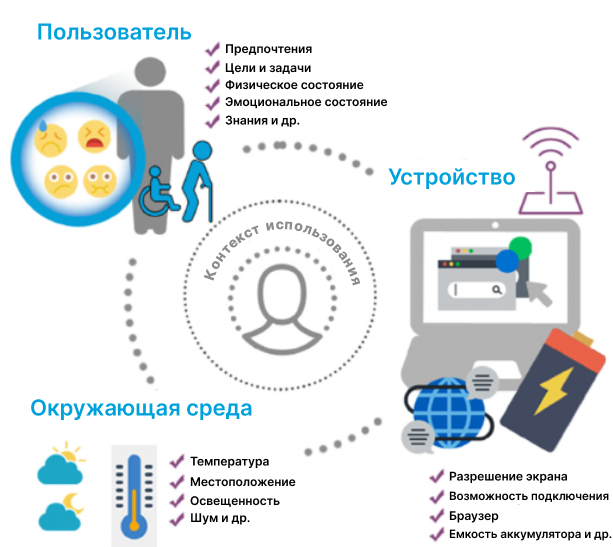
\includegraphics[scale=0.5]{author/part4/figures/user-context.png}
	\caption{Контекст использования системы}
	\label{fig:use_context}
\end{figure}

Настройка функциональных возможностей и параметров интерфейса может осуществляться либо вручную самим пользователем, либо автоматически системой на основании имеющейся информации о пользователе. Таким образом, следует различать адаптивные и адаптируемые системы, эти термины не являются синонимами, хотя в литературе довольно часто можно встретить подмену данных понятий (см. \scncite{Valeev2018}).

В адаптируемых системах любая адаптация является предопределенной и может изменяться пользователями перед запуском системы. В адаптивных же системах, напротив, любая адаптация является динамической, то есть происходит в то же время, когда пользователь взаимодействует с системой, и зависит от поведения пользователя. Но система также может быть адаптируемой и адаптивной одновременно (см. \scncite{Montero2005}).
Недостаток ручного редактирования интерфейса заключается в необходимости пользователя быть достаточно хорошо знакомым, как с самой системой, так и со средствами, позволяющими изменять ее \textit{интерфейс}.

Также в литературе можно встретить термин \textit{``адаптированный интерфейс''}. 

\textit{адаптированный интерфейс} - это \textit{пользовательский интерфейс}, который адаптирован к конечному пользователю при проектировании и не изменяется во время эксплуатации системы (см. \scncite{Schlungbaum1997}).

\textit{интеллектуальный интерфейс} - \textit{пользовательский интерфейс}, который может предположить дальнейшие действия пользователей и представить информацию на основе этого предположения. Можно заметить, что понятия интеллектуальный и адаптивный интерфейс имеют отличия. Однако, в различных статьях эти понятия рассматриваются как синонимы (см. \scncite{Brdnik2022}, \scncite{Volkel2020}, \scncite{Ehlert2003}).

\textit{мультимодальный интерфейс} - \textit{пользовательский интерфейс}, предназначенный для обработки двух или более комбинированных режимов пользовательского ввода, таких как речь, перо, касание, ручные жесты и взгляд, скоординированным образом с выводом мультимедийной системы.

Взаимодействие с большей частью традиционных компьютерных систем происходит с помощью клавиатуры и мыши (тачпада, стилуса). Пользовательский интерфейс таких систем как правило не хранит информацию о модели пользователя, историю его действий и так далее. Традиционный пользовательский интерфейс также не содержит модуль адаптации. На рисунке \nameref{fig:traditional_ui} представлена структура традиционного пользовательского интерфейса (см.\scncite{Sadouski2022}).

\begin{figure}[H]
	\centering
	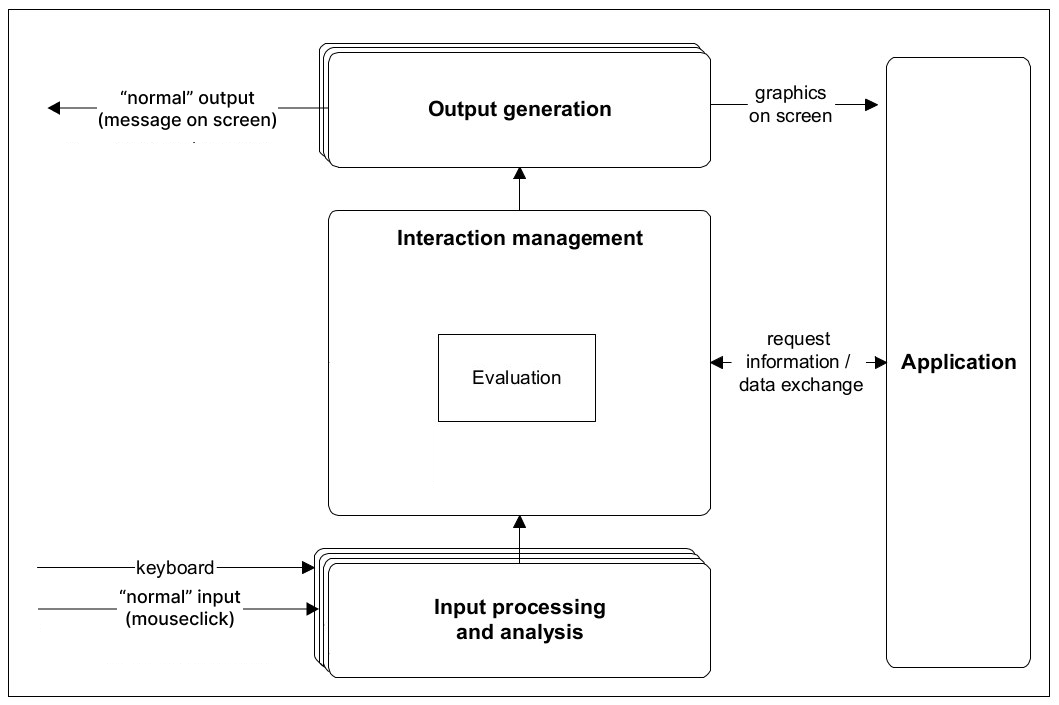
\includegraphics[scale=0.4]{author/part4/figures/traditional_ui.png}
	\caption{Структура традиционного пользовательского интерфейса}
	\label{fig:traditional_ui}
\end{figure}

Общая архитектура адаптивного интеллектуального мультимодального пользовательского интерфейса в свою очередь как правило выглядит так, как представлено на рисунке \nameref{fig:adaptive_ui}.

\begin{figure}[H]
	\centering
	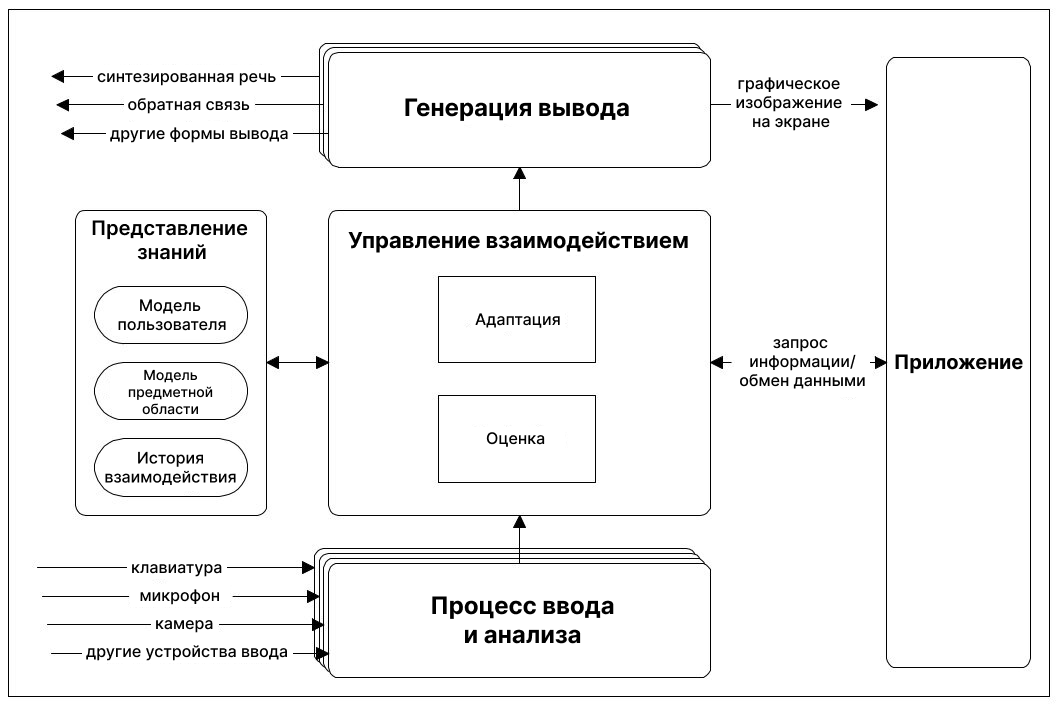
\includegraphics[scale=0.4]{author/part4/figures/adaptive_ui.png}
	\caption{Структура адаптивного интеллектуального мультимодального пользовательского интерфейса}
	\label{fig:adaptive_ui}
\end{figure}

Среди современных средств создания адаптивных пользовательских интерфейсов можно выделить следующие средства, представленные на рисунке \nameref{fig:adaptive_ui_tools} (см. \scncite{Hussain2018}).

\begin{figure}[H]
	\centering
	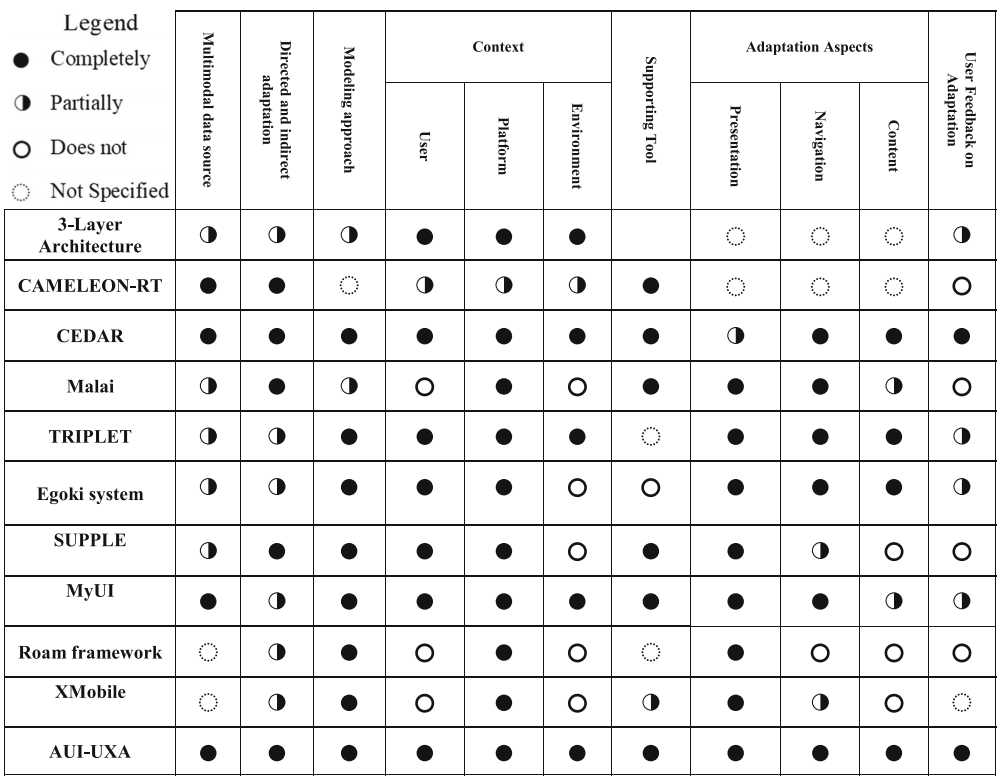
\includegraphics[scale=0.4]{author/part4/figures/adaptive_ui_tools.png}
	\caption{Существующие средства создания адаптивных пользовательских интерфейсов}
	\label{fig:adaptive_ui_tools}
\end{figure}

Вне зависимости от средств создания \textit{адаптивных интеллектуальных мультимодальных пользовательских интерфейсов} такие системы должны эффективно хранить и обрабатывать знания о пользователе, взаимодействии с ним и другую необходимую информацию. Большинство таких систем используют онтологическую модель для хранения информации для адаптации пользовательского интерфейса (см. \scncite{Hitz2016}, \scncite{Liu2005}, \scncite{Gaulke2015}, \scncite{Gribova2011a}, \scncite{Gribova2005}), а также декларативные языки описания \textit{пользовательского интерфейса} (см. \scncite{Abrams1999}, \scncite{Paterno2009}, \scncite{Limbourg2004}, \scncite{Puerta1994}). Именно онтологический подход позволяет:
\begin{textitemize}
	\item создать наиболее полное \myuline{унифицированное описание} различных аспектов пользовательского интерфейса;
	\item \myuline{легко интегрировать} различные аспекты \textit{пользовательского интерфейса};
	\item \myuline{упростить повторное использование} модели интерфейса.
\end{textitemize}

В рамках онтологического подхода принято выделять онтологии и предметные области. База знаний адаптивного интеллектуального мультимодального интерфейса должна включать как минимум следующие предметные области:
\begin{textitemize}
	\item \textit{Предметную область и онтологию модели пользователя}; 
	\item \textit{Предметную область и онтологию компонентов интерфейса};
	\item \textit{Предметную область и онтологию интерфейсных действий};
	\item \textit{Предметную область и онтологию контекста использования}.
\end{textitemize}

Среди существующих \textit{онтологий модели пользователя} можно выделить онтологию GUMO (см. \scncite{Heckmann2007}), в рамках которой выделяют:
\begin{textitemize}
	\item физиологическое состояние - может измениться за секунды;
	\item психическое состояние - может измениться за минуты;
	\item эмоциональное состояние - может измениться за часы;
	\item характер - может измениться за месяцы;
	\item личность - может измениться за годы;
	\item демография - обычно не может измениться.
\end{textitemize}

В работе \scncite{Paulheim2013} рассматривается \textit{онтология компонентов интерфейса}, на верхнем уровне которой рассматриваются следующие типы компонентов:
\begin{textitemize}
	\item компонент пользовательского интерфейса для отображения;
	\item декоративный компонент пользовательского интерфейса;
	\item интерактивный компонент пользовательского интерфейса;
	\item компонент ввода данных;
	\item компонент для манипуляции отображением;
	\item компонент для запуска операций;
	\item контейнер;
	\item окно;
	\item модальное окно;
	\item немодальное окно.
\end{textitemize}

В данную онтологию также можно включить классы свойств компонента, которые определяют оформление внешнего вида интерфейсных элементов, начиная от простых, таких как шрифт, цвет, размер элементов, до составных, содержащих наборы интерфейсных решений (см. \scncite{Gribova2022}).

Классификация \textit{интерфейсных действий} представлена в \scncite{Paulheim2013} и содержит следующие основные классы:
\begin{textitemize}
	\item действие мышью;
	\item действие речью;
	\item действие осязания;
	\item действие прикосновения.
\end{textitemize}


\textit{Онтология контекста использования} рассматривается в работе \scncite{Kong2011} и описывает:
\begin{textitemize}
	\item Статус пользователей:
	\begin{textitemize}
		\item Движение (стояние, сидение, ходьба);
		\item Возможность слушать (да, нет);
		\item Возможность печатать (да, нет);
		\item Возможность говорить (да, нет);
		\item Возможность читать (да, нет);
	\end{textitemize}
	\item Естественная среда:
	\begin{textitemize}
		\item Освещение (яркий, умеренно освещенный, темный);
		\item Шум (шумный, тихий);
		\item Ветер (сильный, слабый, безветрие);
		\item Погода (солнечно, облачно, дождливо);
		\item Температура (жарко, тепло, холодно);
		\item Местоположение (в офисе, в аэропорту, на улице, в библиотеке, дома, в торговом центре);
	\end{textitemize}
	\item Особенности устройства:
	\begin{textitemize}
		\item Размер экрана (большой, маленький);
		\item Тип экрана (монохромный, цветной);
		\item Клавиатура (большая, маленькая, виртуальная).
	\end{textitemize}
\end{textitemize}

Для управления взаимодействием пользователя с системой принято использовать \myuline{интеллектуальные агенты}.

\textit{интеллектуальный агент} способен выполнять гибкое автономное действие для достижения своих целей. Согласно данному определению, гибкость означает:
\begin{textitemize}
	\item Реактивность: интеллектуальные агенты способны воспринимать свою среду и реагировать в своевременном режиме на изменения в ней, чтобы удовлетворить свои цели проектирования;
	\item Проактивность: интеллектуальные агенты способны проявлять целенаправленное поведение, инициируя действия для достижения своих целей проектирования;
	\item Социальная способность: интеллектуальные агенты способны взаимодействовать с другими агентами (и, возможно, людьми) с целью удовлетворения своих целей проектирования.
\end{textitemize}
\textit{интеллектуальные агенты} направлены на единственную цель, но обладают большим знанием о рассуждении в пределах своей деятельности. Умение использовать другие ресурсы (других агентов), предпочтения пользователя или клиента и другие способности являются признаками интеллектуального агента.

В результате проведенного анализа можно сделать следующие выводы:
\begin{textitemize}
	\item Для перехода к \myuline{\textit{парадигме равноправного сотрудничества пользователя и системы}} интерфейсы должны быть адаптивными, интеллектуальными и мультимодальными. Существующие решения позволяют проектировать такие интерфейсы, однако имеют ряд недостатков, которые будут представлены далее.
	\item Структура \textit{интеллектуальных интерфейсов} включает базу знаний, модуль управления взаимодействием пользователя с системой.
	\item При проектировании базы знаний активно применяется онтологический подход и уже реализованы некоторые онтологии, которые используются при проектировании интеллектуальных интерфейсов.
	\item Модуль управления взаимодействием пользователя с системой, как правило, реализуется на основе многоагентного подхода.
\end{textitemize} 

Среди недостатков существующих решений можно выделить:
\begin{textitemize}
	\item Существующие решения, как правило, предусматривают \myuline{вопросно-ответный принцип взаимодействия}.
	\item Актуальной остается \myuline{проблема совместимости интеллектуального интерфейса с интеллектуальной системой}, для которой он создается, в силу различий используемых средств и методов при проектировании и реализации.
	\item Актуальной остается \myuline{проблема совместимости компонентов интеллектуального интерфейса} (база знаний и модуль управления взаимодействием) между собой.
\end{textitemize}

Для устранения недостатков существующих решений предлагается использовать онтологический подход на основе семантической модели при проектировании и реализации \textit{адаптивного интеллектуального мультимодального пользовательского интерфейса}, принципы которого будут рассмотрены далее.

\section{Предлагаемый подход к организации интерфейсов ostis-систем}
\label{sec_proposed_ui_approach}

Для организации \textit{интерфейса ostis-систем} предлагаются следующие принципы:
\begin{textitemize}
	\item Под \textit{пользовательским интерфейсом ostis-системы} понимается специализированная \textit{ostis-система}, ориентированная на решение интерфейсных задач, и имеющая в своем составе базу знаний и решатель задач пользовательского интерфейса ostis-системы (см. \scncite{Boriskin2017}). Таким образом обеспечивается совместимость \textit{ostis-системы} и ее \textit{пользовательского интерфейса}.
	\item Для решения задачи построения пользовательского интерфейса в базе знаний \textit{пользовательского интерфейса ostis-системы} содержится sc-модель \textit{компонентов пользовательского интерфейса}, \textit{интерфейсных действий пользователей}, а также классификация \textit{пользовательских интерфейсов} вцелом.
	\item Решатель задач \textit{пользовательского интерфейса ostis-системы} быть основан на многоагентном подходе, а сами агенты - имеют возможность инициирования действий и сообщений пользователю и другим агентам.
	\item При проектировании \textit{пользовательского интерфейса ostis-системы} используется компонентный подход, который предполагает представление всего интерфейса приложения в виде отдельных специфицированных компонентов, которые могут разрабатываться и совершенствоваться независимо (см. \scncite{Koronchik2011}, \scncite{Koronchik2013}).
	\item Каждый компонент \textit{пользовательского интерфейса ostis-системы} является внешним отображением определенного элемента из базы знаний, что позволяет использовать их в качестве аргументов пользовательских команд и правильно трактовать прагматику и семантику объектов интерфейсной деятельности, легко изменять интерфейс системы даже во время ее эксплуатации, позволяет пользователю задавать системе вопросы касательно любого из компонентов интерфейса.
	\item Модель \textit{пользовательского интерфейса ostis-системы} строится независимо от реализации платформы интерпретации такой модели, что позволяет легко переносить разработанную модель на разные платформы.
	\item Описание модели базы знаний и решателя задач \textit{пользовательского интерфейса ostis-системы} предлагается осуществлять на основе универсального унифицированного языка представления знаний, что обеспечит совместимость между этими компонентами.
\end{textitemize}

\textit{пользовательский интерфейс ostis-системы} является адаптивным интеллектуальным мультимодальным пользовательским интерфейсом, структура которого представлена на рисунке \nameref{fig:ostis_ui_structure} (см. \scncite{Sadouski2021}, \scncite{Sadouski2022b}).

\begin{figure}[H]
	\centering
	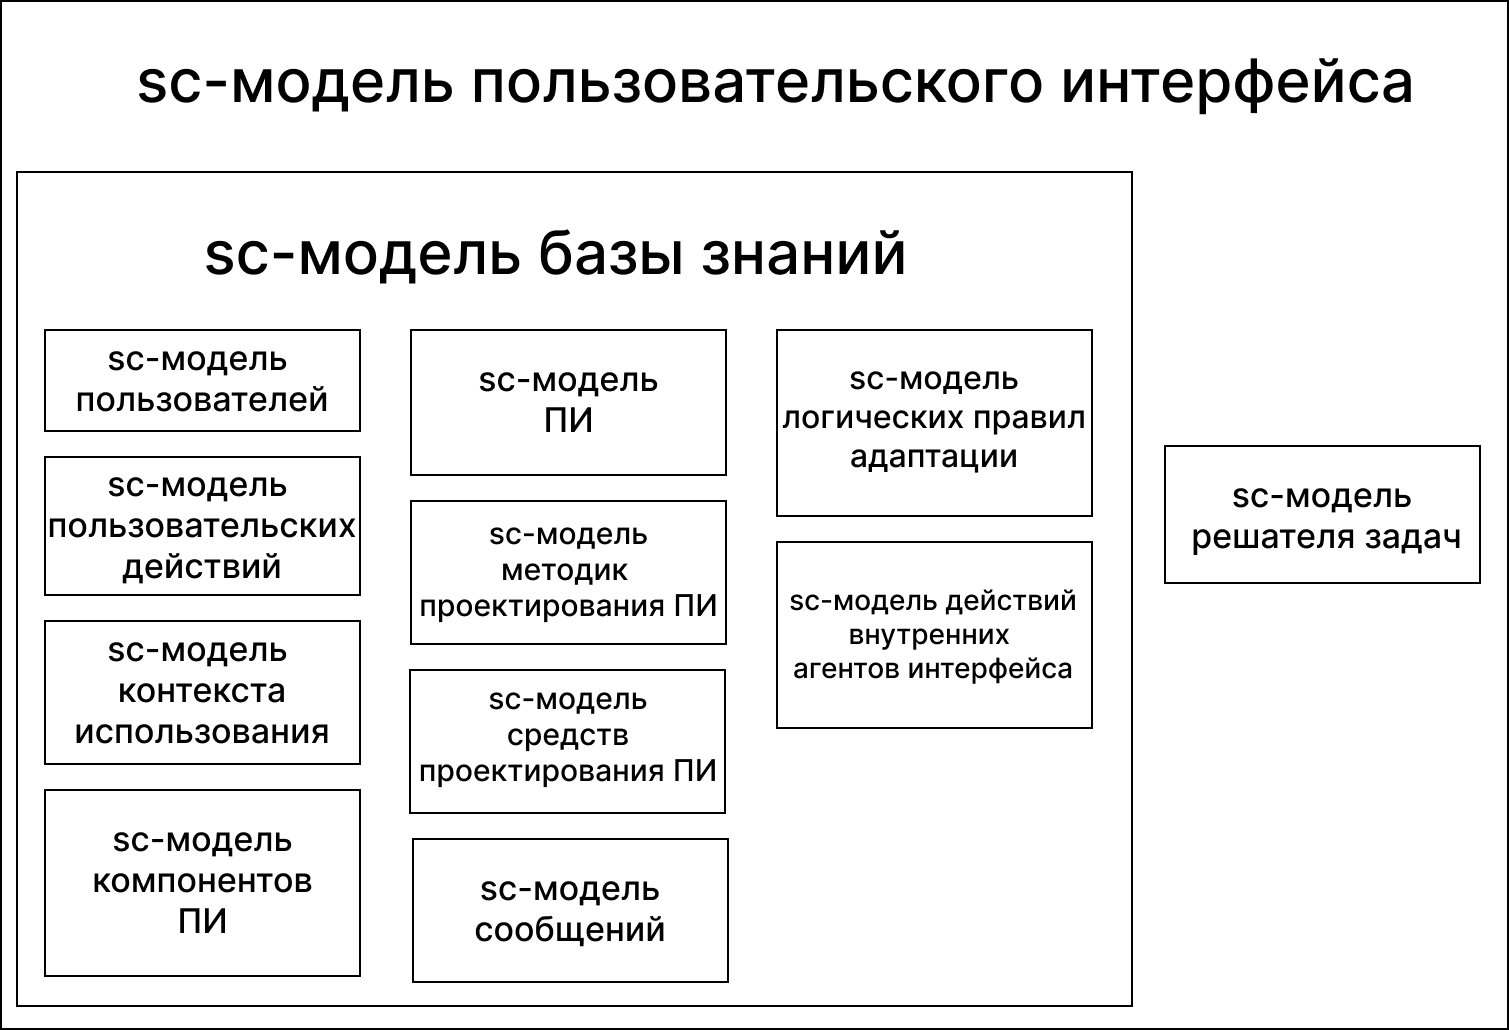
\includegraphics[scale=0.3]{author/part4/figures/ui_model.png}
	\caption{Структура пользовательского интерфейса ostis-системы}
	\label{fig:ostis_ui_structure}
\end{figure}

\textit{Предметная область пользовательских интерфейсов} представляет собой формализованную типологию пользовательских интерфейсов. Пример фрагмента данной предметной области в базе знаний пользовательского интерфейса будет выглядеть следующим образом.

\begin{SCn}
	\scnheader{интерфейс}
	\scnidtf{совокупность технических, программных и методических (протоколов, правил, соглашений) средств, обеспечивающих обмен информацией между пользователем и устройствами и программами, а также между устройствами и другими устройствами и программами. В широком смысле слова, это способ (стандарт) взаимодействия между объектами. Интерфейс в техническом смысле слова задаёт параметры, процедуры и характеристики взаимодействия объектов}
\end{SCn}

\begin{SCn}
	
	\scnheader{интерфейс}
	\begin{scnrelfromset}{разбиение}
			\scnitem{пользовательский интерфейc}
			\begin{scnindent}
					\scnidtf{один из наиболее важных компонентов компьютерной системы. Представляет собой совокупность аппаратных и программных средств, обеспечивающих обмен информацией между пользователем и компьютерной системой.}
				\end{scnindent}
			\scnitem{программный интерфейс}
			\begin{scnindent}
					\scnidtf{система унифицированных связей, предназначенных для обмена информацией между компонентами вычислительной системы. Программный интерфейс задает набор необходимых процедур, их параметров и способов обращения.}
				\end{scnindent}
			\scnitem{физический интерфейс}
			\begin{scnindent}
					\scnidtf{устройство, преобразующее сигналы и передающее их от одного компонента оборудования к другому. Физический интерфейс определяется набором электрических связей и характеристиками сигналов.}
				\end{scnindent}
		\end{scnrelfromset}
	
\end{SCn}

\begin{SCn}
	\scnheader{адаптивный интерфейс}
	\scnidtf{\textit{пользовательский интерфейс}, который изменяется на основе потребностей пользователя или контекста}
\end{SCn}

\begin{SCn}
	\scnheader{интеллектуальный интерфейс}
	\scnidtf{\textit{пользовательский интерфейс}, который может предположить дальнейшие действия пользователей и представить информацию на основе этого предположения}
\end{SCn}

\begin{SCn}
	\scnheader{мультимодальный интерфейс}
	\scnidtf{\textit{пользовательский интерфейс}, предназначенный для обработки двух или более комбинированных режимов пользовательского ввода, таких как речь, перо, касание, ручные жесты и взгляд, скоординированным образом с выводом мультимедийной системы}
\end{SCn}

\begin{SCn}
	
	\scnheader{пользовательский интерфейс}
	\scnsuperset{командный пользовательский интерфейс}
	\begin{scnindent}
			\scnidtf{\textit{пользовательский интерфейс}, при котором обмен информацией между компьютерной системой и пользователем осуществляется путем написания текстовых инструкций или команд}
		\end{scnindent}		
	\scnsuperset{WIMP-интерфейс}
	\begin{scnindent}
			\scnidtf{Window, Image, Menu, Pointer - интерфейс}
			\scnidtf{Окно, Образ, Меню, Указатель - интерфейс}
			\scnidtf{\textit{пользовательский интерфейс}, при котором обмен информацией между компьютерной системой и пользователем осуществляется в форме диалога при помощью окон, меню и других элементов управления}
			\begin{scnindent}
					\scnsuperset{пользовательский интерфейс ostis-системы}
				\end{scnindent}	
		\end{scnindent}
	\scnsuperset{SILK-интерфейс}
	\begin{scnindent}
			\scnidtf{Speech, Image, Language, Knowledge - интерфейс}
			\scnidtf{Речь, Образ, Язык, Знание - интерфейс}
			\scnidtf{\textit{пользовательский интерфейс}, наиболее приближенный к естественной для человека форме общения. Компьютерная система находит для себя команды, анализируя человеческую речь и находя в ней ключевые фразы. Результат выполнения команд преобразуется в понятную человеку форму, например, в естественно-языковую форму или изображение.}
			\scnsuperset{естественно-языковой интерфейc}
			\begin{scnindent}
					\scnidtf{SILK-интерфейс, обмен информацией между компьютерной системой и пользователем в котором происходит за счёт диалога. Диалог ведётся на одном из естественных языков}
				\end{scnindent}			
			\begin{scnindent}
					\scnsuperset{речевой интерфейc}
					\begin{scnindent}
							\scnidtf{SILK-интерфейс, обмен информацией в котором происходит за счёт диалога, в процессе которого компьютерная система и пользователь общаются с помощью речи. Данный вид интерфейса наиболее приближен к естественному общению между людьми}
						\end{scnindent}
				\end{scnindent}
		\end{scnindent}
	
\end{SCn}

\bigskip

\textit{Предметная область пользователя}, \textit{Предметная область контекста использования}, формализована в соотвествии с материалами, рассмотренными в подразделе \nameref{sec_analysis}.

\textit{Предметная область компонентов интерфейса} содержит классификацию компонентов пользовательского интерфейса, пример приведен далее (см. \scncite{Standart2021}).

\begin{SCn}

\scnheader{компонент пользовательского интерфейса}
\scnidtf{знак сущности базы знаний, имеющий определённую форму внешнего представления на экране}
\begin{scnrelfromset}{разбиение}
	\scnitem{атомарный компонент пользовательского интерфейса}
	\begin{scnindent}
		\scnidtf{компонент \textit{пользовательского интерфейса}, не содержащий в своём составе других \textit{компонентов пользовательского интерфейса}}
	\end{scnindent}
	\scnitem{неатомарный компонент пользовательского интерфейса}
		\begin{scnindent}
		\scnidtf{\textit{компонент пользовательского интерфейса}, состоящий из других \textit{компонентов пользовательского интерфейса}}
	\end{scnindent}	
\end{scnrelfromset}

\end{SCn}

\bigskip

\begin{SCn}

\scnheader{визуальная часть пользовательского интерфейса ostis-системы}
\scnidtf{часть базы знаний пользовательского интерфейса ostis-системы, содержащая необходимые для отображения пользовательского интерфейса компоненты}
\scnsubset{неатомарный компонент пользовательского интерфейса}

\end{SCn}

\bigskip
Компоненты пользовательского интерфейса могут быть отнесены к одной из двух категорий: \textit{компонент пользовательского интерфейса для отображения}, \textit{интерактивный компонент пользовательского интерфейса}.

Полная классификация компонентов пользовательского интерфейса приведена далее:
\begin{SCn}

\scnheader{компонент пользовательского интерфейса}
\scnsuperset{интерактивный компонент пользовательского интерфейса}
	\begin{scnindent}
		\scnsuperset{компонент ввода данных}
			\begin{scnindent}
				\scnsuperset{компонент ввода данных с прямой ответной реакцией}
					\begin{scnindent}
						\scnsuperset{область рисования}
						\scnsuperset{ползунок}
						\scnsuperset{компонент ввода текста с прямой ответной реакцией}
							\begin{scnindent}
								\scnsuperset{однострочное текстовое поле}
								\scnsuperset{многострочное текстовое поле}
							\end{scnindent}
						\scnsuperset{компонент выбора}
						\scnrelfrom{разбиение}{Типология компонентов выбора по количеству элементов}
						\begin{scnindent}
							\begin{scneqtoset}
								\scnitem{компонент выбора одного значения}
								\scnitem{компонент выбора нескольких значений}
							\end{scneqtoset}
						\end{scnindent}
						\begin{scnindent}
							\scnsuperset{выбираемый элемент}
							\scnsuperset{радиокнопка}
							\scnsuperset{переключатель}
							\scnsuperset{флаговая кнопка}
						\end{scnindent}
					\end{scnindent}
				\scnsuperset{компонент ввода данных без прямой ответной реакции}
					\begin{scnindent}
						\scnsuperset{кнопка-счётчик}
						\scnsuperset{компонент ввода движений}
						\scnsuperset{компонент речевого ввода}
					\end{scnindent}
			\end{scnindent}
		\scnsuperset{компонент для представления и взаимодействия с пользователем}
			\begin{scnindent}
				\scnsuperset{активирующий компонент}
				\scnsuperset{компонент непрерывной манипуляции}
					\begin{scnindent}
						\scnsuperset{компонент редактирования размера}
						\scnsuperset{полоса прокрутки}
					\end{scnindent}
			\end{scnindent}
		\scnsuperset{компонент запроса действий}
			\begin{scnindent}
				\scnsuperset{компонент выбора команд}
					\begin{scnindent}
						\scnsuperset{пункт меню}
						\scnsuperset{кнопка}
					\end{scnindent}
				\scnsuperset{компонент ввода команд}
			\end{scnindent}
	\end{scnindent}
\scnsuperset{компонент пользовательского интерфейса для отображения}
	\begin{scnindent}
		\scnsuperset{компонент вывода}
			\begin{scnindent}
				\scnsuperset{компонент вывода видео}
				\scnsuperset{компонент вывода звука}
				\scnsuperset{компонент вывода изображения}
				\scnsuperset{компонент вывода графической информации}
					\begin{scnindent}
						\scnsuperset{индикатор выполнения}
						\scnsuperset{диаграмма}
						\scnsuperset{карта}
					\end{scnindent}
				\scnsuperset{компонент вывода текста}
					\begin{scnindent}
						\scnsuperset{сообщение}
						\scnsuperset{заголовок}
						\scnsuperset{параграф}
					\end{scnindent}
			\end{scnindent}
		\scnsuperset{декоративный компонент пользовательского интерфейса}
			\begin{scnindent}
				\scnsuperset{пустое пространство}
				\scnsuperset{разделитель}
			\end{scnindent}
		\scnsuperset{контейнер}
			\begin{scnindent}
				\scnsuperset{списковый контейнер}
				\scnsuperset{древовидный контейнер}
				\scnsuperset{узловой контейнер}
				\scnsuperset{таблично-строковый контейнер}
				\scnsuperset{таблично-клеточный контейнер}
				\scnsuperset{панель вкладок}
				\scnsuperset{панель вращения}
				\scnsuperset{меню}
				\scnsuperset{строка меню}
				\scnsuperset{панель инструментов}
				\scnsuperset{строка состояния}
				\scnsuperset{панель прокрутки}
				\scnsuperset{окно}
					\begin{scnindent}
						\scnsuperset{модальное окно}
						\scnsuperset{немодальное окно}
					\end{scnindent}
			\end{scnindent}
	\end{scnindent}

\end{SCn}

\bigskip

В рамках \textit{Предметной области методик проектирования интерфейсов} предлагается формализовать различные существующие методы проектирования интерфейсов, такие как:
\begin{textitemize}
	\item проектирование пользовательских интерфейсов на основе онтологий(концепция разработки пользовательских интерфйсов на основе онтологий);
	\item методика эргономического проектирования;
	\item методика целеориентированного проектирования.
\end{textitemize}

В рамках \textit{Предметной области средств проектирования интерфейсов} предлагается формализовать существующие средства проектирования интерфейсов (см. \scncite{Myers2001}), такие как:
\begin{textitemize}
	\item средства для поддержки создания интерфейса написанием кода;
	\item интерактивные инструментальные средства;
	\item средства, основанные на создании интерфейса путем связывания отдельно созданных компонентов.
\end{textitemize}

В рамках \textit{Предметной области логических правил адаптации интерфейса} предлагается формализовать типологию логических правил, на основе которых будет происходить адаптация интерфейса к пользователю.

Таким образом, предложена структура \textit{пользовательского интерфейса ostis-системы}, которая включает \textit{базу знаний пользовательского интерфейса ostis-системы} и \textit{решатель задач пользовательского интерфейса ostis-системы}. Рассмотрены \textit{предметные области} в рамках \textit{базы знаний пользовательского интерфейса ostis-системы}. Далее будут подробно рассмотрены классификация \textit{интерфейсных действия пользователей ostis-систем}, \textit{сообщений} и структура \textit{решателя задач пользовательского интерфейса ostis-системы}.

\section{Интерфейсные действия пользователей ostis-систем}
\label{sec_interface_user_actions}


Действие, выполняемое пользователем над некоторым \textit{компонентом пользовательского интерфейса}, называется \textit{интерфейсным действием}. Для связи данного действия с \textit{компонентом пользовательского интерфейса} и необходимым к выполнению \textit{внутренним действием системы} используется отношение \textit{инициируемое пользовательским интерфейсом действие*}.

Классификация интерфейсных действий:

\begin{SCn}

\scnheader{интерфейсное действие пользователя}
\scnsuperset{действие мышью}
\begin{scnindent}
\scnsuperset{прокрутка мышью}
\begin{scnindent}
\scnsuperset{прокрутка мышью вверх}
\scnsuperset{прокрутка мышью вниз}
\end{scnindent}
\scnsuperset{наведение мышью}
\scnsuperset{отпускание мышью}
\scnsuperset{нажатие мыши}
\begin{scnindent}
\scnsuperset{одиночное нажатие мыши}
\scnsuperset{двойное нажатие мыши}			
\end{scnindent}
\scnsuperset{жест мышью}
\scnsuperset{отведение мышью}		
\scnsuperset{перетаскивание мышью}
\end{scnindent}
\scnsuperset{действие голосом}
\scnsuperset{действие клавиатурой}
\begin{scnindent}
\scnsuperset{нажатие функциональной клавиши}
\scnsuperset{нажатие клавиши набора текста}
\end{scnindent}
\scnsuperset{действие осязанием}	
\scnsuperset{действие сенсором}	
\begin{scnindent}
\scnsuperset{нажатие сенсора}
\begin{scnindent}
\scnsuperset{одиночное нажатие сенсора}
\scnsuperset{двойное нажатие сенсора}
\end{scnindent}
\scnsuperset{жест по сенсору}
\begin{scnindent}
\scnsuperset{жест по сенсору одним пальцем}
\scnsuperset{жест по сенсору несколькими пальцами}
\end{scnindent}
\scnsuperset{отпускание сенсором}
\scnsuperset{перетаскивание сенсором}
\end{scnindent}
\scnsuperset{действие пером}	
\begin{scnindent}
\scnsuperset{нажатие функциональной клавиши пером}
\scnsuperset{рисование пером}
\scnsuperset{написание текста пером}
\end{scnindent}

\end{SCn}

\bigskip
\textit{прокрутка мышью} -- интерфейсное действие пользователя, соответствующее прокрутке содержимого некоторого компонента пользовательского интерфейса при помощи мыши.

\textit{наведение мышью} -- интерфейсное действие пользователя, соответствующее появлению курсора мыши в рамках компонента пользовательского интерфейса.

\textit{отпускание мышью} -- интерфейсное действие пользователя, соответствующее отпусканию некоторого компонента пользовательского интерфейса в рамках другого компонента пользовательского интерфейса при помощи мыши.

\textit{нажатие мыши} -- интерфейсное действие пользователя, соответствующее выполнению нажатия мыши в рамках некоторого компонента пользовательского интерфейса.

\textit{отведение мышью} -- интерфейсное действие пользователя, соответствующее выходу курсора мыши за рамки компонента пользовательского интерфейса.

\textit{перетаскивание мышью} -- интерфейсное действие пользователя, соответствующее перетаскиванию компонента пользовательского интерфейса при помощи мыши.

\textit{нажатие сенсора} -- интерфейсное действие пользователя, соответствующее выполнению нажатия сенсора в рамках некоторого компонента пользовательского интерфейса.

\textit{жест по сенсору} -- интерфейсное действие пользователя, соответствующее выполнению некоторого жеста, выполняемого при помощи движения пальцев на экране сенсора.

\textit{отпускание сенсором} -- интерфейсное действие пользователя, соответствующее отпусканию некоторого компонента пользовательского интерфейса в рамках другого компонента пользовательского интерфейса при помощи сенсора.

\textit{перетаскивание сенсором} -- интерфейсное действие пользователя, соответствующее перетаскиванию компонента пользовательского интерфейса при помощи сенсора.

\textit{действие пером} -- интерфейсное действие пользователя, осуществляемое при помощи пера на графическом планшете.

\textit{класс интерфейсных действий пользователя} -- множество, элементами которого являются классы \textit{интерфейсных действий пользователя}.

При взаимодействии пользователя с \textit{компонентом пользовательского интерфейса} могут быть произведены различные \textit{интерфейсные действия}. В зависимости от выполненного \textit{интерфейсного действия} и компонента, над которым оно было выполнено, происходит инициирование некоторого \textit{внутреннего действия системы}. Для задания такого инициируемого при взаимодействии с пользовательским интерфейсом действия и используется указанное отношение. Первым компонентом связки отношения \textit{инициируемое пользовательским интерфейсом действие*} является связка, элементами которой являются элемент множества компонентов пользовательского интерфейса и и элемент множества \textit{класс интерфейсных действий пользователя}. Вторым компонентом является элемент множества \textit{класс внутренних действий системы}.

Таким образом, рассмотрена классификация \textit{пользовательских действий пользователей ostis-системы}, которые могут выполняться в рамках \textit{пользовательского интерфейса ostis-системы}.

\section{Сообщения, входящие в ostis-систему и выходящие из неё}
\label{sec_messages}

\textit{сообщение} -- \textit{дискретная информационная конструкция}, используемая в процессе передачи от отправителя к получателю.

В качестве \textit{отправителя сообщения} может выступать как пользователь системы, так и сама система. В случае ostis-системы сообщение может быть эффекторным либо рецепторным.

\textit{эффекторное сообщение ostis-системы} -- сообщение ostis-системы, формируемое самой ostis-системой при возникновении некоторых ситуаций. К ситуациям, инициирующим возникновение эффекторных сообщений, можно отнести:
\begin{textitemize}
	\item ситуации, возникающие при анализе деятельности самого пользователя. Например, задание аргументов, не соответствующих типу инициируемого действия или появление подсказок при использовании компонентов пользовательского интерфейса;
	\item ситуации, возникающие при анализе синтаксиса текстов внешних языков. Например, неполнота сформированного предложения на внешнем языке или использование конструкций, нехарактерных или некорректно использованных в контексте отдельно взятого внешнего языка/
\end{textitemize}

\textit{рецепторное сообщение ostis-системы} -- сообщение ostis-системы, являющееся реакцией на императивное сообщение (сообщение, побуждающее к какому-либо действию). Возможными реакциями ostis-системы на императивное сообщение пользователя являются:
\begin{textitemize}
	\item указание факта завершения выполнения некоторой задачи, что, например, характерно для поведенческих действий;
	\item получение ответа на поставленную задачу, формируемого либо в результате анализа базы знаний	пользовательского интерфейса, либо в результате анализа предметной части базы знаний самой ostis-системы.
\end{textitemize}

\textit{сообщение пользователя ostis-системы} может быть сформировано как на внешнем языке (языке, внешнем по отношению к ostis-системе, который не используется для коммуникации внутри системы), так и на внутреннем языке (SC-коде).

Любое сообщение может быть атомарным (не содержащем в своем составе другие сообщения) либо неатомарным (сообщение, в состав которого входят другие сообщения).

Типология сообщений представлена в следующем фрагменте:

\begin{SCn}

\scnheader{сообщение}
\begin{scnrelfromset}{разбиение}
\scnitem{сообщение пользователя системы}
\begin{scnindent}
	\scnsubset{сообщение пользователя ostis-системы}
\end{scnindent}
\scnitem{сообщение системы}
\end{scnrelfromset}
\begin{scnrelfromset}{разбиение}
\scnitem{атомарное сообщение}
\scnitem{атомарное сообщение}
\end{scnrelfromset}
\begin{scnrelfromset}{разбиение}
\scnitem{сообщение на естественном языке}
\scnitem{сообщение на искусственном языке}
\end{scnrelfromset}
\scnsubset{графическое сообщение}
\begin{scnindent}
	\scnidtf{сообщение, содержащее графическую информацию}
	\scnsubset{видео-сообщение}
	\begin{scnindent}
		\scnidtf{сообщение, содержащее видео-информацию}
	\end{scnindent}	
\end{scnindent}
\scnsubset{аудио-сообщение}
\begin{scnindent}
	\scnidtf{сообщение, представленное в звуковом формате}
\end{scnindent}
\scnsubset{обонятельное сообщение}
\begin{scnindent}
	\scnidtf{сообщение, содержащее информацию о запахах}
\end{scnindent}
\scnsubset{текстовое сообщение}
\begin{scnindent}
	\scnidtf{сообщение, содержащее текстовую информацию}
\end{scnindent}
\scnsubset{сообщение, требующее трансляции}
\begin{scnindent}
	\scnidtf{сообщение, которое необходимо сформировать системой для дальнейшей передачи его пользователю}
\end{scnindent}
\scnsubset{протранслированное сообщение}
\begin{scnindent}
	\scnidtf{сообщение, которое было сформировано системой для дальнейшей передачи его пользователю}
\end{scnindent}

\end{SCn}

Таким образом, рассмотрена типология \textit{сообщений}, которые являются основой взаимодействия пользователя с \textit{интерфейсом} системы.

\section{Действия и внутренние агенты пользовательского интерфейса ostis-системы}
\label{sec_interfaces_actions_and_agents}

\textit{решатель задач пользовательского интерфейса ostis-систем} состоит из некоторого коллектива \textit{sc-агентов}, обеспечивающих работу пользователя с \textit{компонентами пользовательского интерфейса ostis-системы}.

При использовании \textit{sc-агентов} стоит помнить различия в \myuline{семантической} и \myuline{прагматической} составляющей любого \textit{компонента пользовательского интерфейса}. \myuline{Семантическая составляющая} заключается в определении того, знаком какой сущности является отображаемый на экране компонент. \myuline{Прагматическая составляющая} рассматривает прикладной аспект (аспект применения) отображаемого на экране компонента.

На уровне \textit{sc-памяти} имеет значение только \myuline{семантическая составляющая}, однако данный факт не влияет на процесс эксплуатации системы пользователем, поскольку обе составляющие отражают разные стороны одного и того же знака некоторой сущности. Например, за каждой кнопкой скрывается знак некоторого \textit{класса действия}, инициируемого при нажатии на кнопку. Таким образом, \textit{интерфейсное действие пользователя}, как правило, инициирует некоторое \textit{внутреннее действие системы}. 

\begin{SCn}

\scnheader{внутреннее действие системы}
\scnsuperset{внутреннее действие ostis-системы}

\scnheader{внутреннее действие ostis-системы}
\scnidtf{действие в sc-памяти}
\scnidtf{действие, выполняемое в sc-памяти}

\end{SCn}
	
Каждое \textit{внутреннее действие ostis-системы} обозначает некоторое преобразование, выполняемое некоторым \textit{sc-агентом} (или коллективом \textit{sc-агентов}) и ориентированное на преобразование \textit{sc-памяти}.

\begin{SCn}

\scnheader{действие в sc-памяти}
\scnsuperset{действие в sc-памяти, инициируемое вопросом}
\scnsuperset{действие редактирования базы знаний ostis-системы}
\scnsuperset{действие установки режима ostis-системы}
\scnsuperset{действие редактирования файла, хранимого в sc-памяти}
\scnsuperset{действие интерпретации программы, хранимой в sc-памяти}

\end{SCn}

\bigskip

С точки зрения обработки модели \textit{базы знаний пользовательского интерфейса ostis-систем} должны быть решены следующие задачи:
\begin{textitemize}
	\item обработка пользовательских действий;
	\item интерпретация модели \textit{базы знаний пользовательского интерфейса ostis-системы} (построение \textit{пользовательского интерфейса});
\end{textitemize}

Таким образом, в \textit{решателе задач пользовательского интерфейса ostis-систем} можно выделить \textit{интерпретатор sc-моделей пользовательских интерфейсов} и \textit{интерпретатор пользовательских действий}.

\textit{интерпретатор sc-моделей пользовательских интерфейсов} в качестве входного параметра принимает экземпляр \textit{компонента пользовательского интерфейса} для отображения. При этом компонент может быть как атомарным, так и неатомарным (например, компонент главного окна приложения). Результатом работы интерпретатора является графическое представление указанного компонента с учетом используемой реализации \textit{платформы интерпретации семантических моделей ostis-систем}.

Алгоритм работы данного \textit{интерпретатора} следующий (см. \scncite{Sadouski2022}):
\begin{textitemize}
	\item проверяется тип входного \textit{компонента пользовательского интерфейса} (атомарный или неатомарный);
	\item если \textit{компонент пользовательского интерфейса} является атомарным, то отобразить его графическое представление на основании указанных для него свойств. В случае, если данный компонент не входит в \textit{декомпозицию} любого другого \textit{компонента пользовательского интерфейса} - завершить выполнение. Иначе определить компонент, в \textit{декомпозицию} которого входит рассматриваемый \textit{компонент пользовательского интерфейса}, применить его свойства для текущего атомарного компонента и начать обработку найденного неатомарного компонента, перейдя к первому пункту;
	\item если \textit{компонент пользовательского интерфейса} является неатомарным, то проверить, были ли отображены компоненты, на которые он был декомпозирован. Если да, то завершить выполнение, иначе определить еще не отображенный компонент из декомпозиции обрабатываемого неатомарного компонента и начать обработку найденного компонента, перейдя к первому пункту.
\end{textitemize}

\textit{интерпретатор пользовательских действий} является \textit{неатомарным sc-агентом}, который включает в себя множество \textit{sc-агентов}, каждый из которых обрабатывает \textit{интерфейсные действия пользователя} определенного класса (например, \textit{абстрактный sc-агент обработки действия нажатия мыши}, \textit{абстрактный sc-агент обработки действия отпускания мыши} и так далее). Интерпретатор реагирует на появление в базе знаний системы экземпляра \textit{интерфейсного действия пользователя}, находит связанный с ним класс \textit{внутреннего действия} и генерирует экземпляр данного \textit{внутреннего действия} для последующей обработки.

Таким образом, предложена структура \textit{решателя задач пользовательского интерфейса ostis-систем}, которая позволяет обеспечить работу пользователя с \textit{компонентами пользовательского интерфейса ostis-системы}.

\section*{Заключение к Главе~\ref{chapter_interfaces}}

В главе были рассмотрены принципы организации \myuline{партнёрского взаимодействия пользователя с интеллектуальной системой} и принципы построения \textit{интерфейсов интеллектуальных компьютерных систем нового поколения}, обеспечивающих переход к \myuline{парадигме равноправного сотрудничества}.

В результате проведенного анализа были сделаны следующие выводы:
\begin{textitemize}
	\item Для перехода к \myuline{парадигме равноправного сотрудничества пользователя и системы} интерфейсы должны быть \myuline{адаптивными, интеллектуальными и мультимодальными}. Существующие решения позволяют проектировать такие интерфейсы, однако имеют ряд недостатков.
	\item Структура \textit{интеллектуальных интерфейсов} включает базу знаний, модуль управления взаимодействием пользователя с системой.
	\item При проектировании базы знаний активно применяется онтологический подход и уже реализованы некоторые онтологии, которые используются при проектировании \textit{интеллектуальных интерфейсов}.
	\item Модуль управления взаимодействием пользователя с системой, как правило, реализуется на основе многоагентного подхода.
\end{textitemize} 

Среди недостатков существующих решений были выделены:
\begin{textitemize}
	\item Существующие решения, как правило, предусматривают \myuline{вопросно-ответный принцип взаимодействия}. 
	\item Актуальной остается проблема \myuline{совместимости интеллектуального интерфейса с интеллектуальной системой}, для которой он создается, в силу различий используемых средств и методов при проектировании и реализации.
	\item Актуальной остается проблема \myuline{совместимости компонентов интеллектуального интерфейса} (база знаний и модуль управления взаимодействием) между собой.
\end{textitemize}

Предложен \myuline{онтологический подход на основе семантической модели} к проектированию и реализации \textit{адаптивного интеллектуального мультимодального пользовательского интерфейса} на основе \textit{Технологии  OSTIS}, который позволит обеспечить:
\begin{textitemize}
	\item \myuline{совместимость интеллектуального интерфейса с интеллектуальной системой};
	\item \myuline{совместимость компонентов интеллектуального интерфейса} между собой;
	\item \myuline{взаимодействие пользователя с системой} через \textit{интеллектуальный интерфейс} на \myuline{равноправной основе}.
\end{textitemize}
Предложена и рассмотрена структура \textit{пользовательского интерфейса ostis-системы} и составляюшие ее компоненты.

%%%%%%%%%%%%%%%%%%%%%%%%% referenc.tex %%%%%%%%%%%%%%%%%%%%%%%%%%%%%%
% sample references
% %
% Use this file as a template for your own input.
%
%%%%%%%%%%%%%%%%%%%%%%%% Springer-Verlag %%%%%%%%%%%%%%%%%%%%%%%%%%
%
% BibTeX users please use
% \bibliographystyle{}
% \bibliography{}
%
\biblstarthook{In view of the parallel print and (chapter-wise) online publication of your book at \url{www.springerlink.com} it has been decided that -- as a genreral rule --  references should be sorted chapter-wise and placed at the end of the individual chapters. However, upon agreement with your contact at Springer you may list your references in a single seperate chapter at the end of your book. Deactivate the class option \texttt{sectrefs} and the \texttt{thebibliography} environment will be put out as a chapter of its own.\\\indent
References may be \textit{cited} in the text either by number (preferred) or by author/year.\footnote{Make sure that all references from the list are cited in the text. Those not cited should be moved to a separate \textit{Further Reading} section or chapter.} If the citatiion in the text is numbered, the reference list should be arranged in ascending order. If the citation in the text is author/year, the reference list should be \textit{sorted} alphabetically and if there are several works by the same author, the following order should be used:
\begin{enumerate}
\item all works by the author alone, ordered chronologically by year of publication
\item all works by the author with a coauthor, ordered alphabetically by coauthor
\item all works by the author with several coauthors, ordered chronologically by year of publication.
\end{enumerate}
The \textit{styling} of references\footnote{Always use the standard abbreviation of a journal's name according to the ISSN \textit{List of Title Word Abbreviations}, see \url{http://www.issn.org/en/node/344}} depends on the subject of your book:
\begin{itemize}
\item The \textit{two} recommended styles for references in books on \textit{mathematical, physical, statistical and computer sciences} are depicted in ~\cite{science-contrib, science-online, science-mono, science-journal, science-DOI} and ~\cite{phys-online, phys-mono, phys-journal, phys-DOI, phys-contrib}.
\item Examples of the most commonly used reference style in books on \textit{Psychology, Social Sciences} are~\cite{psysoc-mono, psysoc-online,psysoc-journal, psysoc-contrib, psysoc-DOI}.
\item Examples for references in books on \textit{Humanities, Linguistics, Philosophy} are~\cite{humlinphil-journal, humlinphil-contrib, humlinphil-mono, humlinphil-online, humlinphil-DOI}.
\item Examples of the basic Springer style used in publications on a wide range of subjects such as \textit{Computer Science, Economics, Engineering, Geosciences, Life Sciences, Medicine, Biomedicine} are ~\cite{basic-contrib, basic-online, basic-journal, basic-DOI, basic-mono}. 
\end{itemize}
}

\begin{thebibliography}{99.}%
% and use \bibitem to create references.
%
% Use the following syntax and markup for your references if 
% the subject of your book is from the field 
% "Mathematics, Physics, Statistics, Computer Science"
%
% Contribution 
\bibitem{science-contrib} Broy, M.: Software engineering --- from auxiliary to key technologies. In: Broy, M., Dener, E. (eds.) Software Pioneers, pp. 10-13. Springer, Heidelberg (2002)
%
% Online Document
\bibitem{science-online} Dod, J.: Effective substances. In: The Dictionary of Substances and Their Effects. Royal Society of Chemistry (1999) Available via DIALOG. \\
\url{http://www.rsc.org/dose/title of subordinate document. Cited 15 Jan 1999}
%
% Monograph
\bibitem{science-mono} Geddes, K.O., Czapor, S.R., Labahn, G.: Algorithms for Computer Algebra. Kluwer, Boston (1992) 
%
% Journal article
\bibitem{science-journal} Hamburger, C.: Quasimonotonicity, regularity and duality for nonlinear systems of partial differential equations. Ann. Mat. Pura. Appl. \textbf{169}, 321--354 (1995)
%
% Journal article by DOI
\bibitem{science-DOI} Slifka, M.K., Whitton, J.L.: Clinical implications of dysregulated cytokine production. J. Mol. Med. (2000) doi: 10.1007/s001090000086 
%
\bigskip

% Use the following (APS) syntax and markup for your references if 
% the subject of your book is from the field 
% "Mathematics, Physics, Statistics, Computer Science"
%
% Online Document
\bibitem{phys-online} J. Dod, in \textit{The Dictionary of Substances and Their Effects}, Royal Society of Chemistry. (Available via DIALOG, 1999), 
\url{http://www.rsc.org/dose/title of subordinate document. Cited 15 Jan 1999}
%
% Monograph
\bibitem{phys-mono} H. Ibach, H. L\"uth, \textit{Solid-State Physics}, 2nd edn. (Springer, New York, 1996), pp. 45-56 
%
% Journal article
\bibitem{phys-journal} S. Preuss, A. Demchuk Jr., M. Stuke, Appl. Phys. A \textbf{61}
%
% Journal article by DOI
\bibitem{phys-DOI} M.K. Slifka, J.L. Whitton, J. Mol. Med., doi: 10.1007/s001090000086
%
% Contribution 
\bibitem{phys-contrib} S.E. Smith, in \textit{Neuromuscular Junction}, ed. by E. Zaimis. Handbook of Experimental Pharmacology, vol 42 (Springer, Heidelberg, 1976), p. 593
%
\bigskip
%
% Use the following syntax and markup for your references if 
% the subject of your book is from the field 
% "Psychology, Social Sciences"
%
%
% Monograph
\bibitem{psysoc-mono} Calfee, R.~C., \& Valencia, R.~R. (1991). \textit{APA guide to preparing manuscripts for journal publication.} Washington, DC: American Psychological Association.
%
% Online Document
\bibitem{psysoc-online} Dod, J. (1999). Effective substances. In: The dictionary of substances and their effects. Royal Society of Chemistry. Available via DIALOG. \\
\url{http://www.rsc.org/dose/Effective substances.} Cited 15 Jan 1999.
%
% Journal article
\bibitem{psysoc-journal} Harris, M., Karper, E., Stacks, G., Hoffman, D., DeNiro, R., Cruz, P., et al. (2001). Writing labs and the Hollywood connection. \textit{J Film} Writing, 44(3), 213--245.
%
% Contribution 
\bibitem{psysoc-contrib} O'Neil, J.~M., \& Egan, J. (1992). Men's and women's gender role journeys: Metaphor for healing, transition, and transformation. In B.~R. Wainrig (Ed.), \textit{Gender issues across the life cycle} (pp. 107--123). New York: Springer.
%
% Journal article by DOI
\bibitem{psysoc-DOI}Kreger, M., Brindis, C.D., Manuel, D.M., Sassoubre, L. (2007). Lessons learned in systems change initiatives: benchmarks and indicators. \textit{American Journal of Community Psychology}, doi: 10.1007/s10464-007-9108-14.
%
%
% Use the following syntax and markup for your references if 
% the subject of your book is from the field 
% "Humanities, Linguistics, Philosophy"
%
\bigskip
%
% Journal article
\bibitem{humlinphil-journal} Alber John, Daniel C. O'Connell, and Sabine Kowal. 2002. Personal perspective in TV interviews. \textit{Pragmatics} 12:257--271
%
% Contribution 
\bibitem{humlinphil-contrib} Cameron, Deborah. 1997. Theoretical debates in feminist linguistics: Questions of sex and gender. In \textit{Gender and discourse}, ed. Ruth Wodak, 99--119. London: Sage Publications.
%
% Monograph
\bibitem{humlinphil-mono} Cameron, Deborah. 1985. \textit{Feminism and linguistic theory.} New York: St. Martin's Press.
%
% Online Document
\bibitem{humlinphil-online} Dod, Jake. 1999. Effective substances. In: The dictionary of substances and their effects. Royal Society of Chemistry. Available via DIALOG. \\
http://www.rsc.org/dose/title of subordinate document. Cited 15 Jan 1999
%
% Journal article by DOI
\bibitem{humlinphil-DOI} Suleiman, Camelia, Daniel C. O'Connell, and Sabine Kowal. 2002. `If you and I, if we, in this later day, lose that sacred fire...': Perspective in political interviews. \textit{Journal of Psycholinguistic Research}. doi: 10.1023/A:1015592129296.
%
%
%
\bigskip
%
%
% Use the following syntax and markup for your references if 
% the subject of your book is from the field 
% "Computer Science, Economics, Engineering, Geosciences, Life Sciences"
%
%
% Contribution 
\bibitem{basic-contrib} Brown B, Aaron M (2001) The politics of nature. In: Smith J (ed) The rise of modern genomics, 3rd edn. Wiley, New York 
%
% Online Document
\bibitem{basic-online} Dod J (1999) Effective Substances. In: The dictionary of substances and their effects. Royal Society of Chemistry. Available via DIALOG. \\
\url{http://www.rsc.org/dose/title of subordinate document. Cited 15 Jan 1999}
%
% Journal article by DOI
\bibitem{basic-DOI} Slifka MK, Whitton JL (2000) Clinical implications of dysregulated cytokine production. J Mol Med, doi: 10.1007/s001090000086
%
% Journal article
\bibitem{basic-journal} Smith J, Jones M Jr, Houghton L et al (1999) Future of health insurance. N Engl J Med 965:325--329
%
% Monograph
\bibitem{basic-mono} South J, Blass B (2001) The future of modern genomics. Blackwell, London 
%
\end{thebibliography}
